\chapter{Results and Discussion}

\section{Termination Step of P3HT Synthesis}

The first problem tackled in this project was to develop an inline procedure for properly terminating the polymerisation prior to passing it through the separation and analysis stages of the flow reactor. Small amounts of unreacted Grignard monomer in the reaction mixture can cause the polymerisation to continue once the droplets have left the oil bath, causing the polymer chain length to increase during the analysis step. This leads to unreliable measurements, and at high molecular weights can cause precipitation of the product polymer inside the GPC column, causing blockages (which require multiple cleaning washes to remove) or even breaking the elution chamber.

Initially, the introduction of a wash was considered. The wash solvent ideally would be able to extract the unreacted Grignard species from the THF phase, and be immiscible with THF itself. However, it was crucial not to introduce a wash that caused precipitation of the polymer out of the THF phase. The use of ionic liquids (ILs) was investigated, with a paper published by O. Kuzmina et. al. and the thesis of P. J. Corbytt showing the ability of the ionic liquid 1-butyl-3-methylimidazolium acetate ([bmim][OAc]) to remove group 1 and transition metal salts from solution, with the aim to remove any leftover unreacted Grignard reagent from solution. However, due to the amount of IL needed to wash the reaction mixture over an extended period, the cost and volume of waste produced would be too high for an efficient continuous process. Therefore, alternative methods were investigated.

The introduction of a solution of a non-selective GRIM catalyst could potentially be used to react together any unused monomers, including the minority isomer that leads to undesirable couplings. The resultant formation of dithiophene in the reaction mixture was not expected to interfere with the analysis due to its very low molecular weight.  

To form solely dithiophene molecules instead of longer chain oligomers, the catalyst should be added in excess compared to the number of unreacted monomers left in solution. The concentration of catalyst needed to obtain a 1:1 ratio of monomer unit to active non-selective catalyst centre for a completely unreacted monomer solution was calculated assuming the same flow rate of the non-selective catalyst solution as the Ni(dppp)Br2 solution, shown in Figure 15. 



\subsection{Production of Non-Selective Catalyst Solution}

The active non-selective catalyst must be formed in solution due to its low solubility in THF. Different target concentrations of Ni(TPP)2Br2 were attempted to be made by adding different quantities of Ni(dme)Br2 and TPP to THF under inert conditions. A summary of the results can be seen in Table 1 below.

\begin{table}[]
	\begin{tabular}{llll}
		Catalyst Loading /mol \% & Ni(dme)Br2 /g & PPh3 /g & Notes         \\
		50                       & 0.386         & 0.918   & Not dissolved \\
		15                       &               &         & Dissolved    
	\end{tabular}
\end{table}

A molar ratio of at least 3:1 TPP to Ni(dme)Br2 was used to shift the ligand exchange equilibrium towards the bis-triphosphino complex. The X M solution was selected for use as it dissolved completely, and contained sufficient Ni(TPP)2Br2 catalyst to fully quench all active species in the monomer solution.

\subsection{Testing of Reaction Termination}

To test whether the Ni(TPP)2Br2 solution would indeed terminate the GRIM reaction, a batch synthesis of P3HT was performed as outlined in the experimental section. At regular time intervals aliquots of the reaction mixture were withdrawn from the reaction flask with a syringe, and quenched in acidified methanol to cause precipitation of the product P3HT. The result can be seen in Figure 14 below.

\includegraphics{AliquotQuick}

Initially the molecular weight of the P3HT was observed to increase at an approximately constant rate of X/min. However, after approximately six minutes the reaction slowed considerably, consistent with the quasi-living chain growth mechanism, described in Chapter 1. The reaction was then repeated with a more dilute reaction, by halving the concentration of the reagents as so to increase the duration of the “living” growth phase with a view to allowing sufficient time for Ni(TPP)2Br2 addition in later experiments. The results are shown in Figure 15.

\includegraphics{AliquotLong}

Under the diluted conditions used, the “living” growth phase lasted approximately ten minutes, sufficiently long for Ni(TPP)2Br2 addition. The reaction was then repeated with the same conditions, but a solution of Ni(TPP)2Br2 was injected into the flask at the five-minute mark. The result can be seen in Figure 16.

\includegraphics{AliquotTermination}

Upon injection of the catalyst solution, the molecular weight of P3HT plateaued at just over 32 kDa, and did not increase further over a period of ninety minutes, indicating that the reaction had successfully been terminated. The high value of Mn obtained on the 5-minute mark occurred because the withdrawn aliquot was held in the syringe longer whilst the catalyst solution was injected into the reaction flask, leaving the polymer to grow for a longer time before being quenched.

\subsection{Introduction of Termination Step in Flow}

Once the ability to terminate the polymerisation reaction was shown, it was implemented into the droplet flow reactor. The previous reactor setup was modified to include an additional flow mixer, as shown in Figure 17.

\includegraphics{HerringtonReactor}
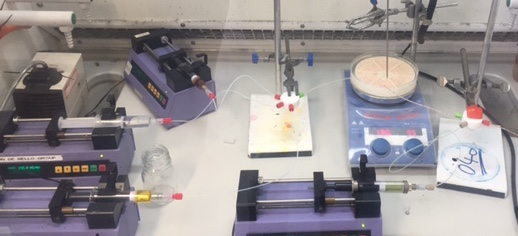
\includegraphics{JackReactor}

To determine whether the termination would supress unwanted coupling and precipitation inside the GPC column, a droplet flow synthesis was run over an extended time, and monitored periodically via the GPC instrument to show long term stability. The transmission response for each successive GPC trace can be seen in Figure 18.

\includegraphics{2hours}

Each GPC analysis takes 15 minutes to run to completion, and the reaction was run for 75 minutes, allowing for five successive analyses to be completed. All the traces show 2 distinct peaks at X and Y, as opposed to the desired single peak, indicative of polymer samples of two separate lengths, which may have arisen from termination step causing the synthesis of short chain oligomers from the remaining monomer in solution. The signals vary in intensity, which indicates that the different samples injected had different concentrations of P3HT. The yellow trace shows additional noise following the expected signal. This occurred due to the improper separation of the two-phase droplet flow, resulting in the inclusion of some Galden in the GPC sample. This issue required a more in-depth look at the liquid-liquid separator and monitoring of the separation quality, as so to prevent future contamination of the GPC column.

\section{Liquid-Liquid Separator Design}

The initial design of the liquid-liquid droplet flow separator was proposed by Dr James Bannock, seen in Figure 19. 

\includegraphics{sepjames}
\includegraphics{bannockseparatoroperation}

The separator consists of two “terminal” blocks made from aluminium or PTFE with channels milled out to form a T-junction. The two blocks are joined by a 4 mm ID diameter tube. A smaller tube with OD 2 mm of partially permeable PFPE capillary tubing runs through the centre to form a tube-in-tube system. On either end of the two PTFE blocks, tubing of ID 1mm leaves the separator. A micro-metering needle valve is attached to one end of the separator to provide back pressure to the system and so coax part of the liquid into passing through the porous wall of the tubing.

The separation occurs due to differences in the wettability of the two liquids to the partially permeable tubing. The liquid that wets most readily to the tubing will travel through the pores of the wall at a lower system pressure than the other liquid. By providing a back pressure to the system between these two pressures, one liquid will be forced through the porous wall of the tubing whilst the other will flow through.

The assembly of a separator involved a fiddly procedure to prevent leakage of the reaction stream, due to the large number of connecting nuts and ferrules (outlined in the experimental section). Higher back pressures often resulted in leaks, limiting the operating range of the system. Furthermore, because of the assembly method required the use of tweezers to pull the porous capillary through each terminal block, the partially permeable tubing was prone to being stretched, changing the effective pore size of the material. This resulted in significant performance from one separator to the next. 
To alleviate these problems, the separator was redesigned to be made from a single PTFE block, as shown in Figure 20. A photograph of the completed block in operation can be seen underneath the design schematic.

\includegraphics{jackseparator1}

Unlike the previous separator, the PFPE stream was removed through a central connection as opposed to at either end of the separator. The device still provided an ample separation window for a THF:PFPE droplet phase system whilst allowing for a much easier assembly process.
As mentioned in section X, with the old separator, some PFPE occasionally leaked into the GPC column due to imperfect separation voiding the analysis at that time and risking damage to the column. Furthermore, in the instance of a fault somewhere in the system that may lead to the incorrect functioning of the separator, the ability to automatically prevent the introduction of incorrect material into the GPC would be an important safely measure. Therefore, a method of flagging instances of improper separation is an important consideration for a fully automated system.

To determine the phase separation of the two output streams, a setup was built to monitor phase separation within the tubing. A photodiode was used to detect the change in transmitted light from an LED as a result of the changing liquid phase within the tubing. A diagram of the operating principle can be seen in Figure 21.

\includegraphics{Photodiode}

The separator design was modified to allow optical detection as soon as possible after the separated streams are isolated. A schematic and picture of the new separator can be seen in Figure 22.

\includegraphics{}

The outlet stream that has passed through the porous tube enters a 2 mm channel. A photodiode and LED lie perpendicularly to this channel, with the light from the LED passing through the 2 mm channel and then onto an OPT 101 monolithic photodiode. The output stream that does not pass through the porous capillary first is removed from the block in 1 mm ID PTFE tubing, which is shaped as a U-bend and re-enters the block. The tubing passes perpendicularly through a 2 mm channel which an LED shines directly onto an OPT 101 monolithic photodiode. A diagram of the circuit setup can be seen in the appendix of this report. 

To test the ability of the separator to correctly identify phase change in the outlet streams, a simple system to mimic the flow reactor was set up. P3HT was dissolved in THF and pumped into a flow mixer at a flow rate equal to that used in the reactor setup. A second syringe pump introduced a stream of PFPE into the mixer, forming a droplet phase system of THF and PFPE. The droplet flow was then fed directly into the separator. A picture of the setup can be seen in Figure 23.

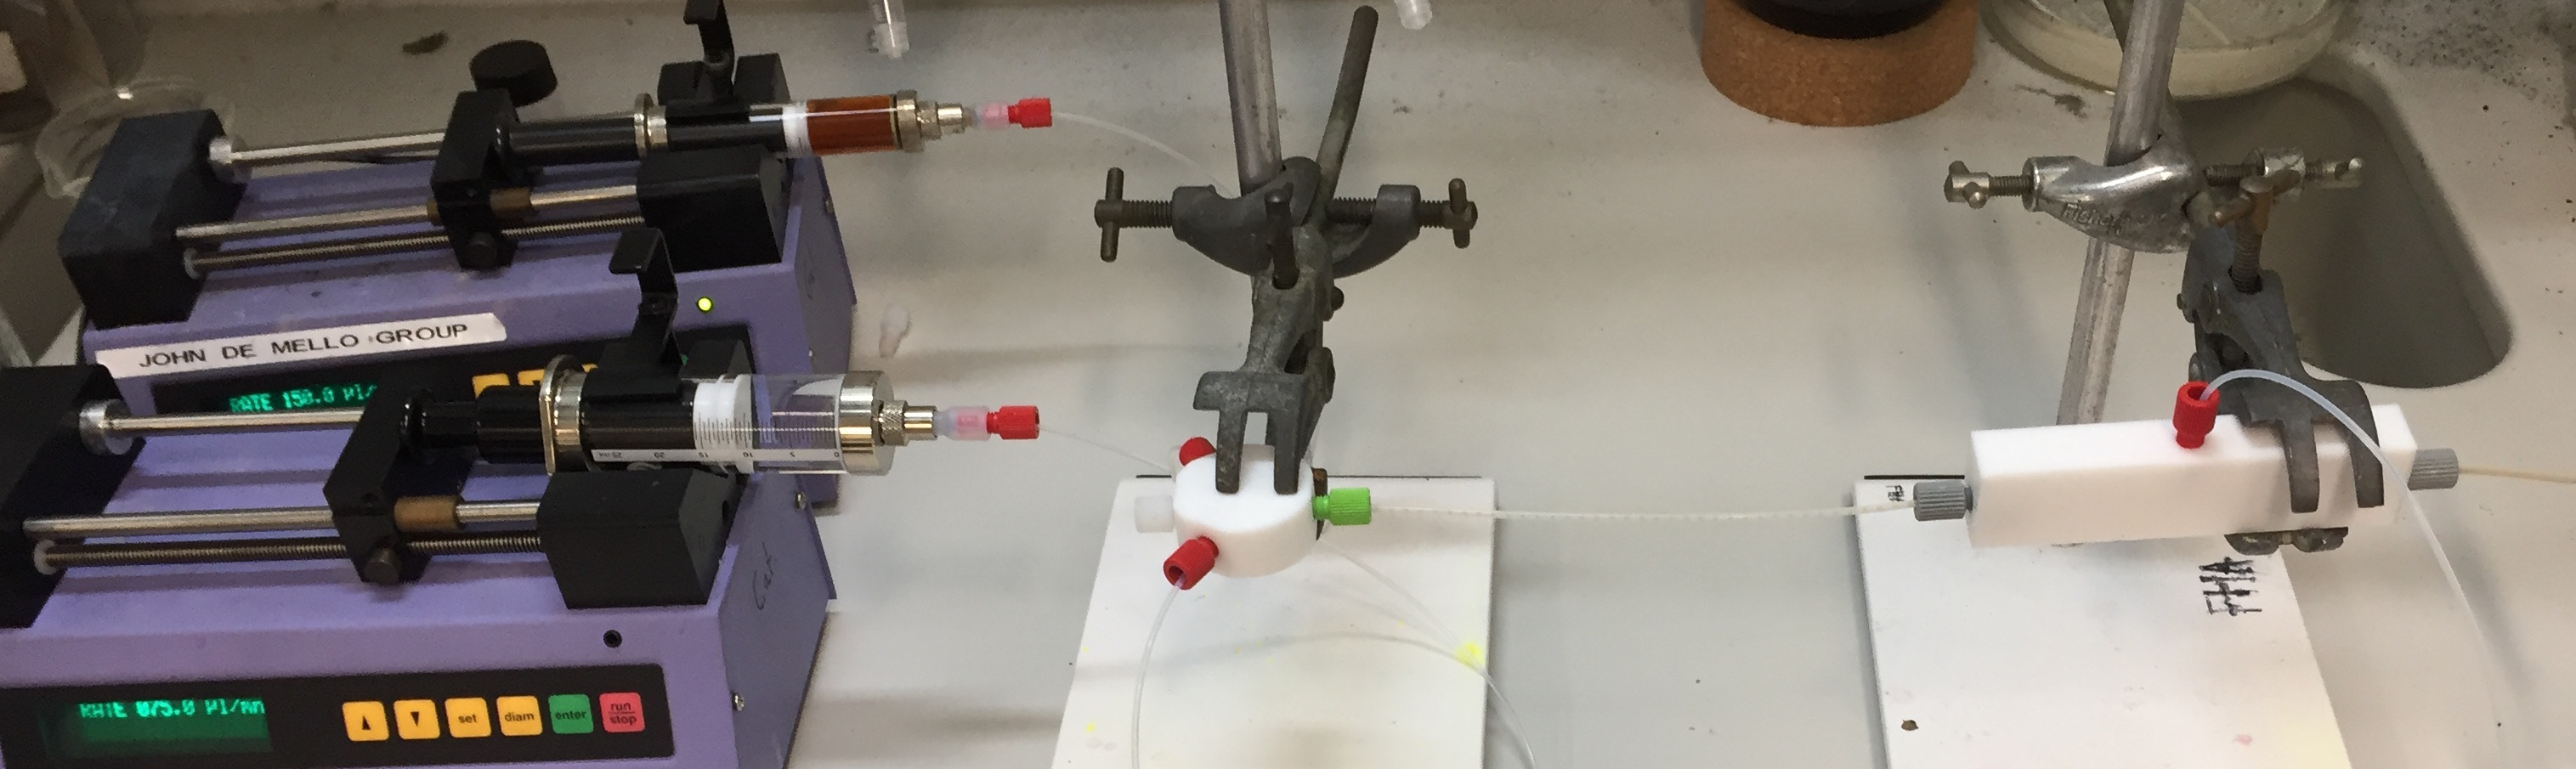
\includegraphics{SepSetup}

An example transmission response of one of the two outlet streams can be seen in Figure 24, showing the clear sensitivity upon changing phase. 

\includegraphics{PDResponse}

\section{GPC Calibration}

The GPC calibrated according to the procedure outlined in Section 1 of this report. A set of nine polymer standards of varying molecular weights and narrow PDs were required. A set of P3HT samples synthesised throughout the project were selected as the standards, and their properties as measured on a commercial GPC are outlined in the Table 2 below.

\begin{table}[]
	\begin{tabular}{llll}
		& Mn    & Mw     & PD     \\
		J1 & 36633 & 61012  & 1.6655 \\
		J2 & 75704 & 141420 & 1.8681 \\
		J3 & 15022 & 18586  & 1.2373 \\
		J4 & 58235 & 111045 & 1.9068 \\
		J5 & 52275 & 129472 & 2.4767 \\
		J6 & 35368 & 56372  & 1.5939 \\
		J7 & 78877 & 133990 & 1.6987 \\
		J8 & 15230 & 18829  & 1.2363 \\
		J9 & 24052 & 36344  & 1.311 
	\end{tabular}
\end{table}

The values obtained for these samples were taken by a refractive index detector. In the current prototype GPC system, a transmission spectrum is taken using a light source at X nm. A comparison of the trace taken on the commercial GPC instrument and the prototype instrument can be seen in Figure 25.

\includegraphics{calibj2}

\includegraphics{J2Graph}

The signal profile is not the same between the two, with the commercial GPC signal consisting of a single peak, whereas the prototype GPC shows a smaller should following the strongest signal. This indicates that the signals display different molecular weight dynamics, and so the maximum signal of one trace cannot be said to correspond to the maximum signal of the other. Whilst it would be better to exchange the detection system to match the commercial instrument’s RI measurement, the current method can still provide a ball-park figure of the molecular weight dynamics of the sample injected.  As outlined in the literature, it is necessary for the samples used in a calibration set to have a narrow PD, ideally less than 1.2. As evident from Table 2, the samples used had a wide range of PDs. Whilst this reduces the accuracy of the calibration, the samples were selected on the basis that the time taken to synthesise a large selection of P3HT samples of low PD was not possible in the time frame available for this project.

The samples were dissolved in THF, and run through the column. Each trace obtained can be found in the appendix. A summary of each sample and their corresponding peak retention time can be seen in Table 3. 

\begin{table}[]
	\begin{tabular}{lll}
		& Peak Retention Time & Mw     \\
		J1 & 6.35835             & 61012  \\
		J2 & 5.95835             & 141420 \\
		J3 & 6.81668             & 18586  \\
		J4 & 6.06668             & 111045 \\
		J5 & 6.01668             & 129472 \\
		J6 & 6.39168             & 56372  \\
		J7 & 6.71668             & 133990 \\
		J8 & 5.77502             & 18829  \\
		J9 & 6.39168             & 36344 
	\end{tabular}
\end{table}

From this data, a calibration curve was plotted for the prototype GPC instrument (see Fig. 26). The corresponding highest and lowest retention times for the calibration set are 6.81 min and 5.96 min which give a calibration window of 18 kDa to 141 kDa. As polymers of high Mw are prone to precipitation out of solution in the reactor, the calibration provides a more than ample analysis range of relevance to the system.

\includegraphics{CalibrationCurve}

To test the calibration, multiple syntheses were run on the system to show whether the system could accurately identify the Mw of synthesised polymer. 




